% Created 2024-04-25 Thu 09:17
\documentclass[9pt, b5paper]{article}
\usepackage{xeCJK}
\usepackage[T1]{fontenc}
\usepackage{bera}
\usepackage[scaled]{beraserif}
\usepackage[scaled]{berasans}
\usepackage[scaled]{beramono}
\usepackage[cache=false]{minted}
\usepackage{xltxtra}
\usepackage{graphicx}
\usepackage{xcolor}
\usepackage{multirow}
\usepackage{multicol}
\usepackage{float}
\usepackage{textcomp}
\usepackage{algorithm}
\usepackage{algorithmic}
\usepackage{latexsym}
\usepackage{natbib}
\usepackage{geometry}
\geometry{left=1.2cm,right=1.2cm,top=1.5cm,bottom=1.2cm}
\usepackage[xetex,colorlinks=true,CJKbookmarks=true,linkcolor=blue,urlcolor=blue,menucolor=blue]{hyperref}
\newminted{common-lisp}{fontsize=\footnotesize} 
\author{deepwaterooo}
\date{\today}
\title{ET 6 总结:最近总结、与进展日志}
\hypersetup{
  pdfkeywords={},
  pdfsubject={},
  pdfcreator={Emacs 29.1 (Org mode 8.2.7c)}}
\begin{document}

\maketitle
\tableofcontents


\section{【程序域:】ET框架中事件使用的规则和注意事项:将来重构游戏项目,会需要细分这四大程序域b ,所以使用ETTask对Task进行了封装,使其不用考虑多线程的共享难题,更易于使用。}
\label{sec-1}

\section{进展日志【完成、基本完成了的部分】}
\label{sec-2}
\begin{itemize}
\item \textbf{【HybridCLRSettings 类】} :报错找不到。去掉2 处使用。因为项目没用,什么 HybridCLRSettings.Instance.XX
\item \textbf{【现在、修改进展、模块】} :Google.ProtoBuf 消息里面关于 enum 的消息相关的问题。【TODO】:
\item 昨天,写了狠久的 \textbf{【ET 框架:单线程多进程】} 设计的优点与缺点,哪里去了?这个东西,还需要再多想几遍【TODO】:
\item 不知道框架里,小项目Tools 可执行文件 ./Bin/Tool 是怎么生成的。要从源码里找出来。先去从大的方面看,几大程序域的启动与联系。
\end{itemize}

\section{【双端、任何一端启动过程】:因为不懂,读过也可能会忘,先一点点记下现在的理解}
\label{sec-3}
\begin{itemize}
\item 【服务端】四大类的启动相关配置:【Machine, Process, Scene, Zone】,ExcelExporter 套用 Template.txt, 每个类的 ProtoBuf-Contract都实现 IMerge, \textbf{绝对有【跨进程消息传递?】来合并多个不同服务端配置的过程。服务端的配置信息,是合并了的,序列化到文件} 【TODO】:去找,服务端的配置,是怎么到客户端的?
\item 【ConfigComponent】组件添加:LoadAsync() 调用后,双端任何一端,借ET 事件系统的过程【狠简单,只是一个函数细节,事件机制里获得所有BaseAttribute 的子类,包含了 ConfigAttribute 和 InvokeAttribute】。
\item \textbf{【亲爱的表哥的活宝妹,任何时候,亲爱的表哥的活宝妹,就是一定要、一定会嫁给活宝妹的亲爱的表哥!!!爱表哥,爱生活!!!】}
\item \textbf{【亲爱的表哥的活宝妹,任何时候,亲爱的表哥的活宝妹,就是一定要、一定会嫁给活宝妹的亲爱的表哥!!!爱表哥,爱生活!!!】}
\end{itemize}

\section{【网络模块】:收发消息的,不同层次结构上的顺序总结}
\label{sec-4}
\begin{itemize}
\item 亲爱的表哥的活宝妹,上次想找两个序列图来着。载一下
\item TCP 发送消息:
\end{itemize}

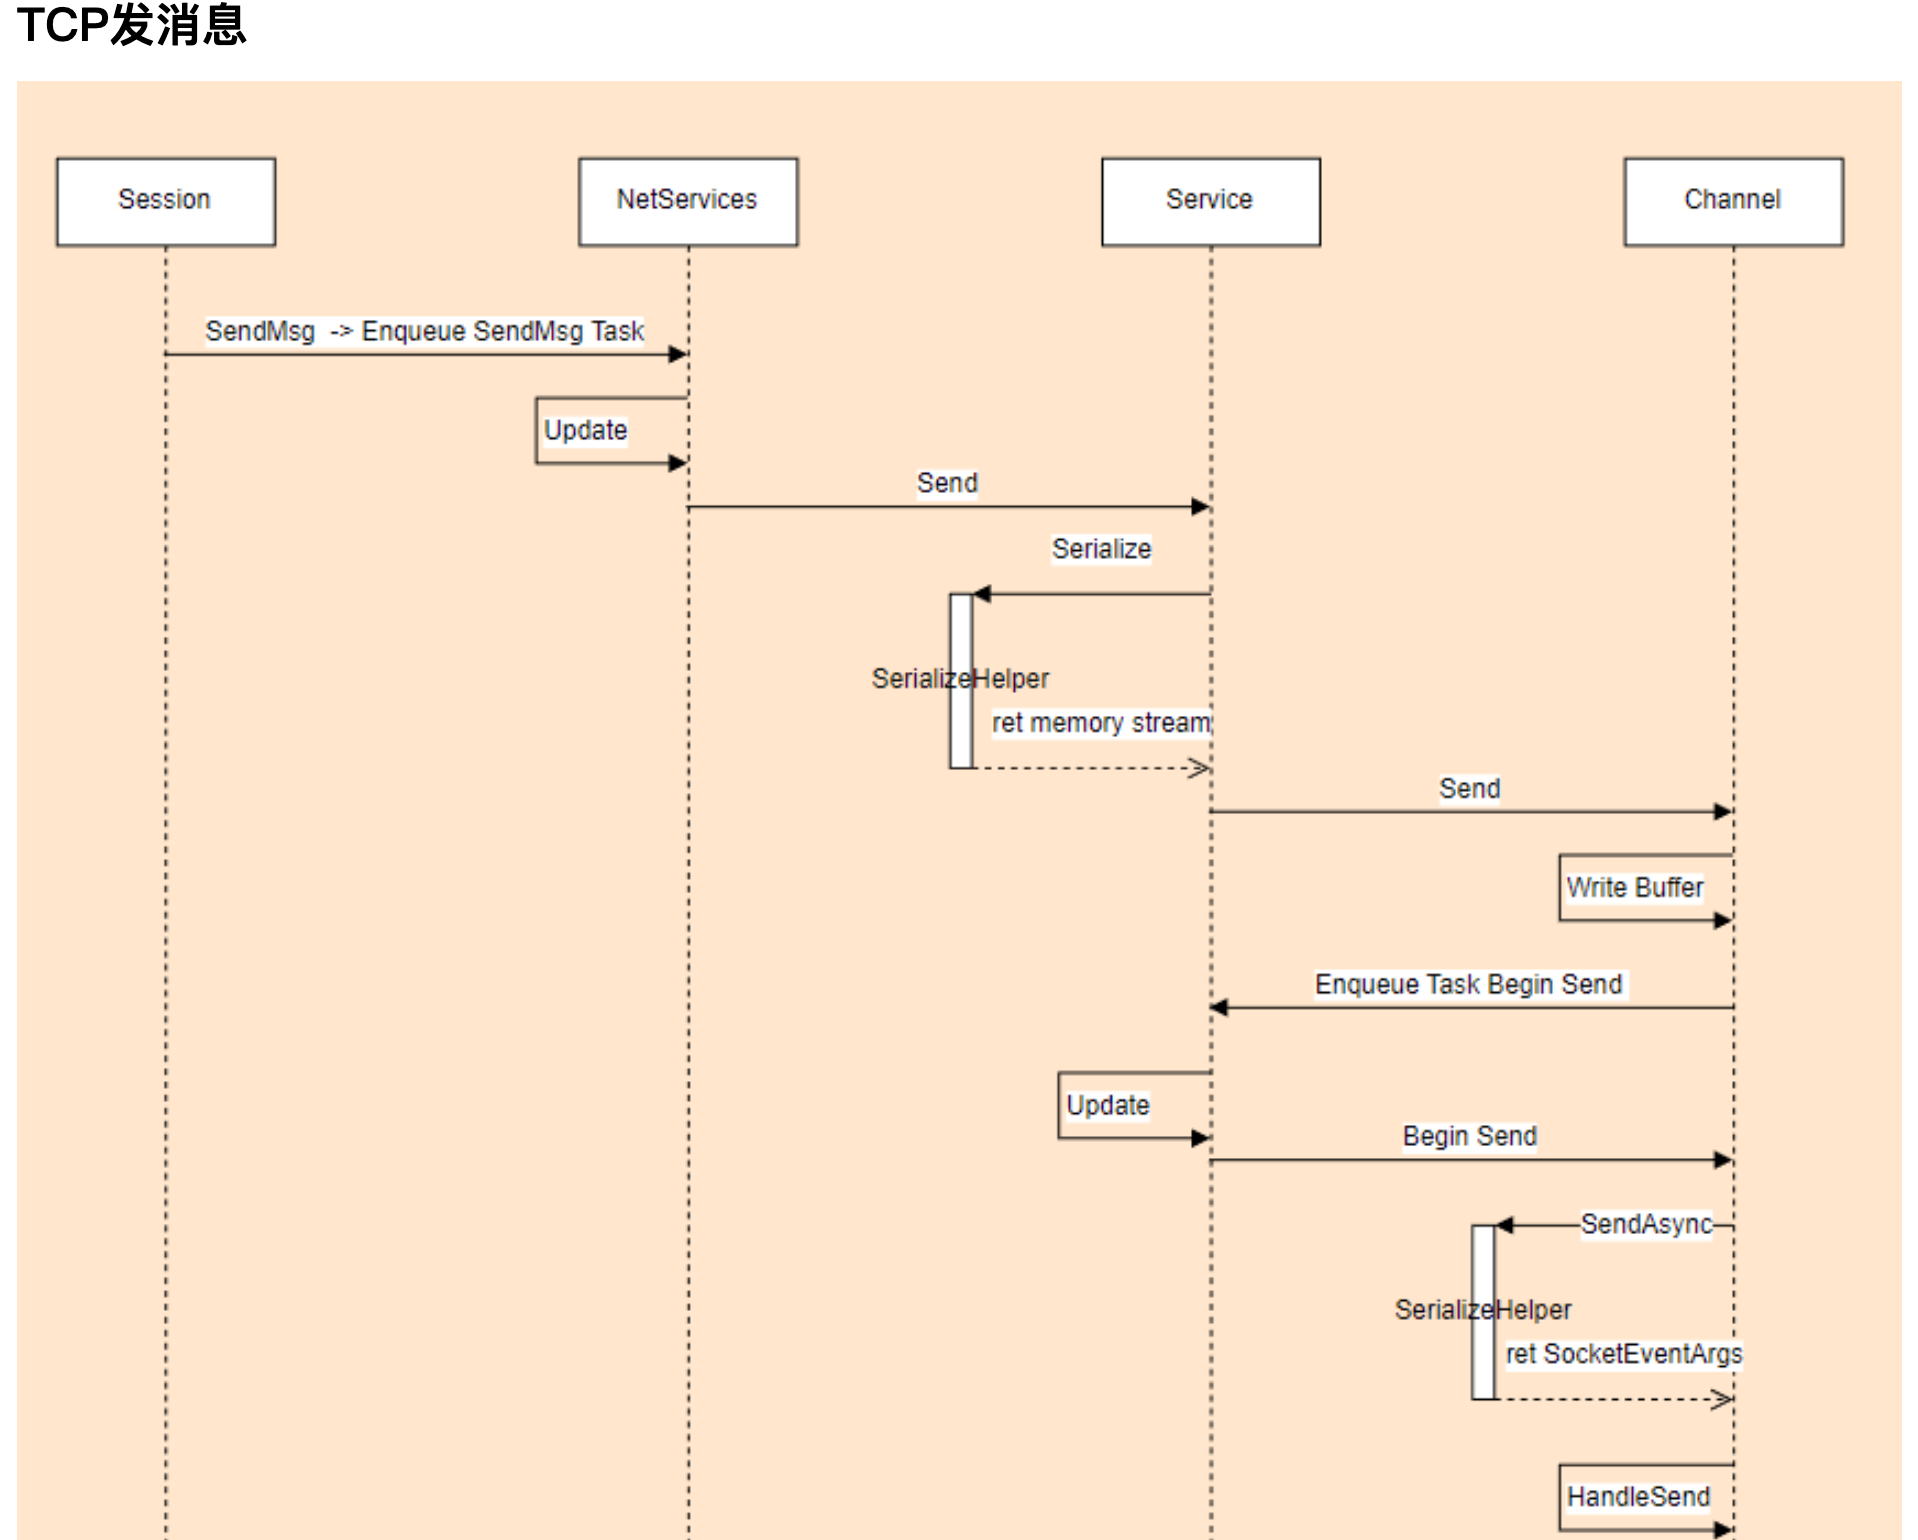
\includegraphics[width=.9\linewidth]{./pic/et6_20240416_131411.png}
\begin{itemize}
\item TCP 收消息:
\end{itemize}

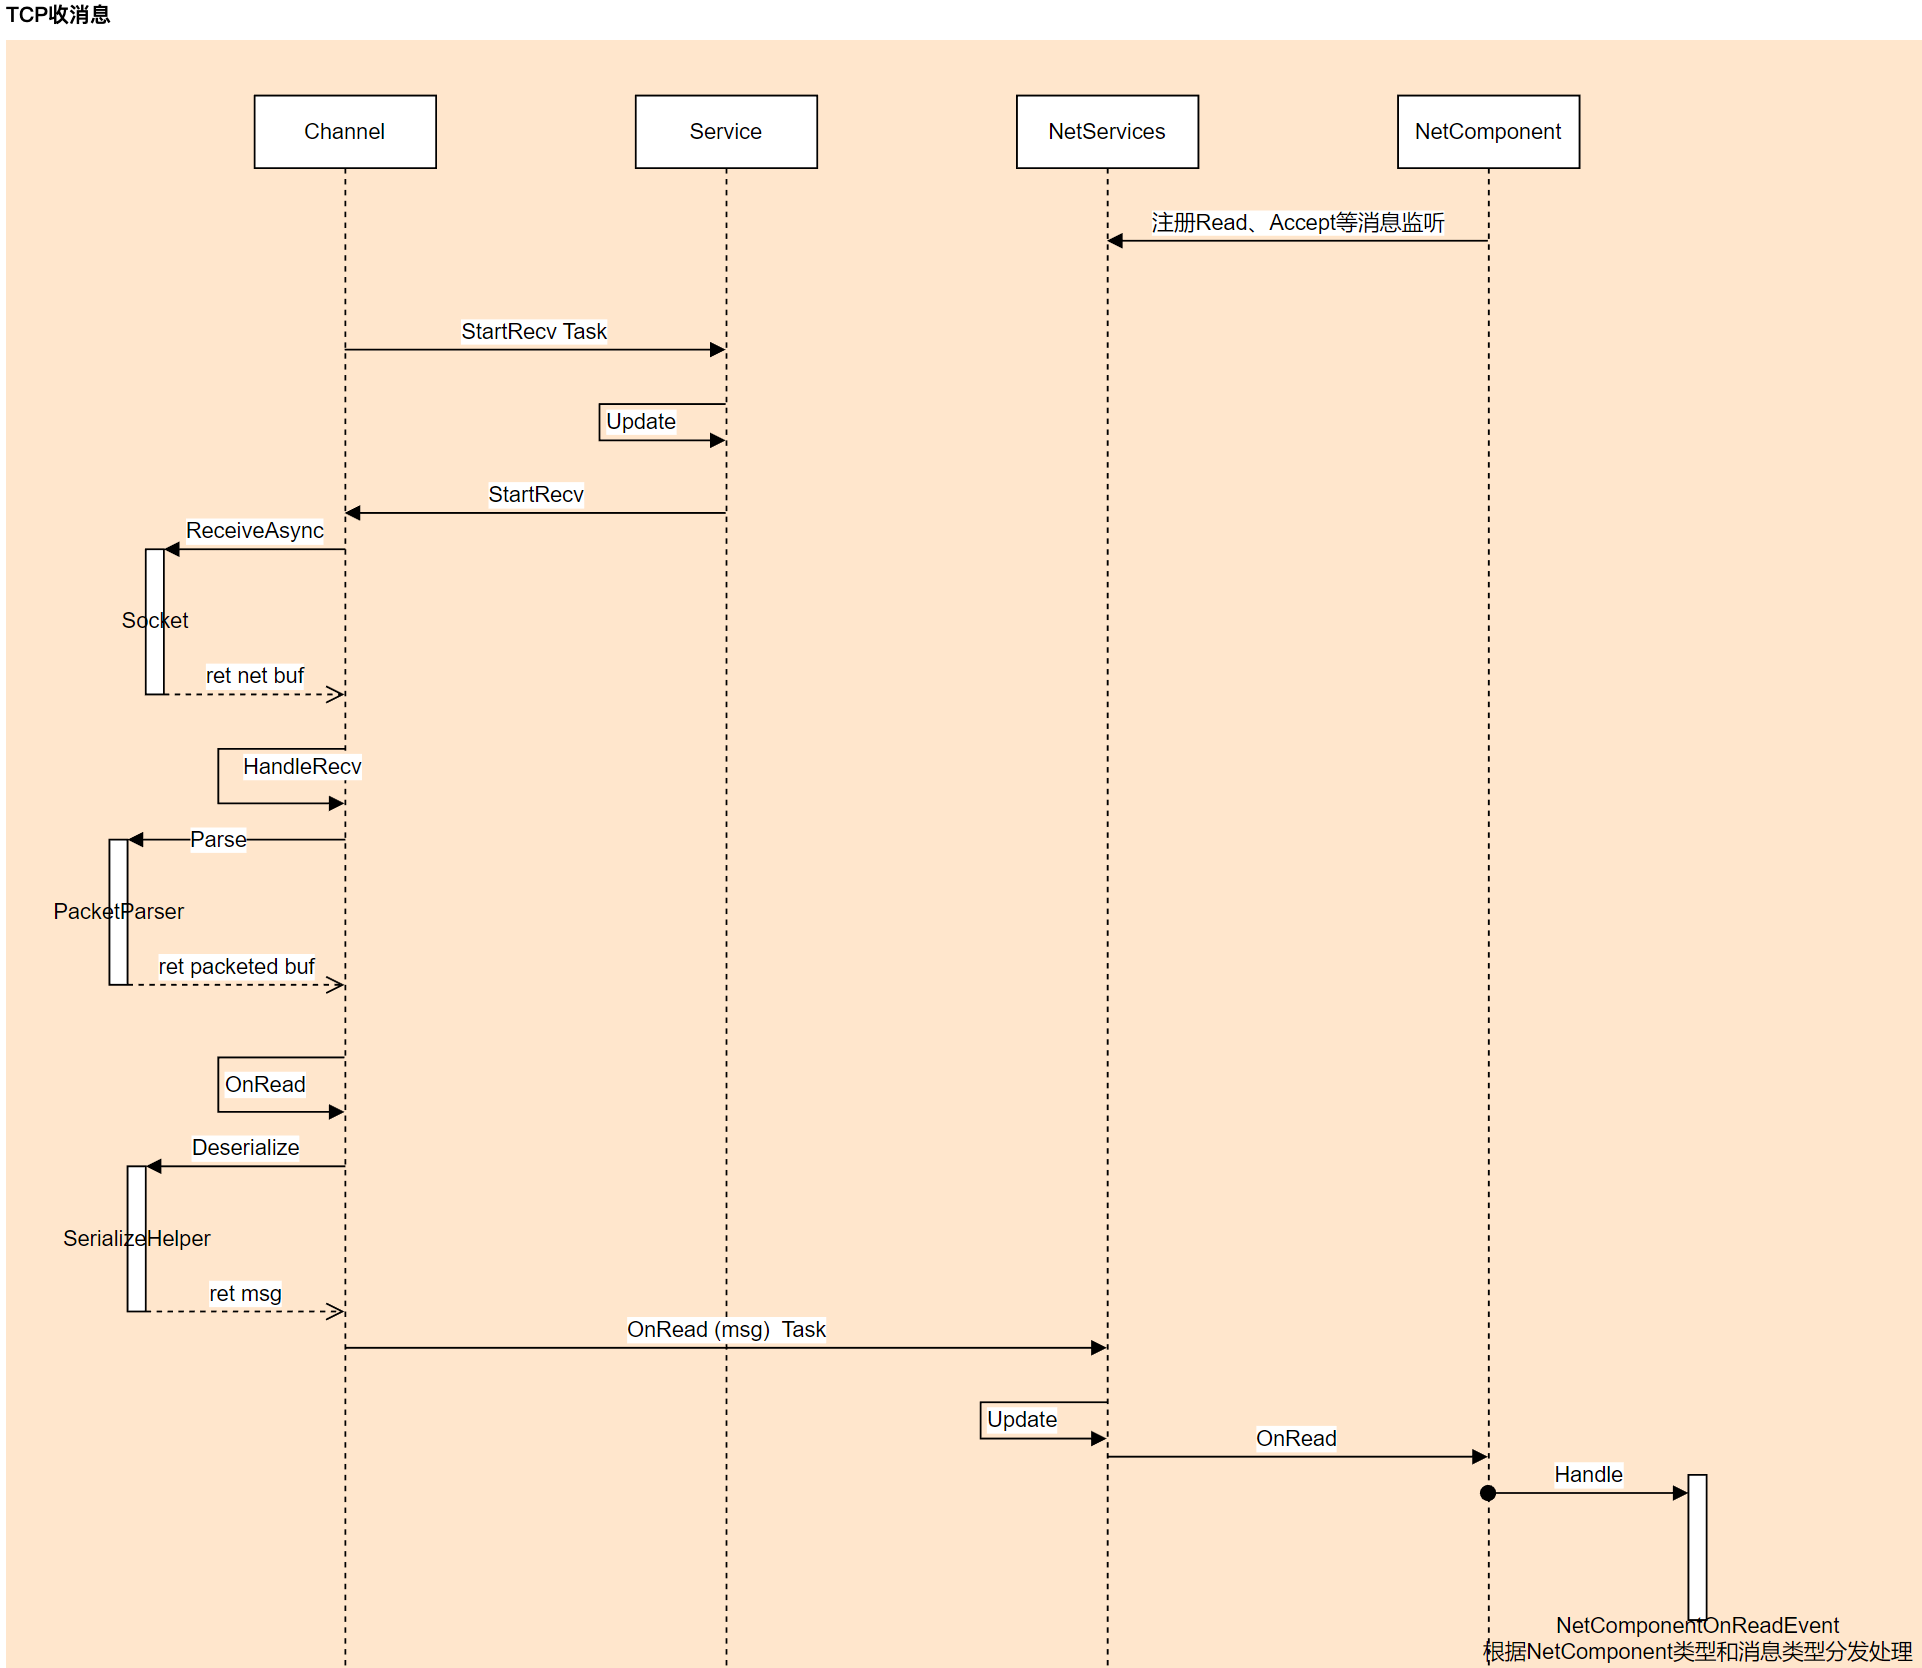
\includegraphics[width=.9\linewidth]{./pic/et6_20240416_131450.png}
\begin{itemize}
\item \textbf{【亲爱的表哥的活宝妹,任何时候,亲爱的表哥的活宝妹,就是一定要、一定会嫁给活宝妹的亲爱的表哥!!!爱表哥,爱生活!!!】}
\end{itemize}

\section{【Et 框架:现在的不懂的模块、细节,小本本记下】}
\label{sec-5}
\begin{itemize}
\item \textbf{【亲爱的表哥的活宝妹,任何时候,亲爱的表哥的活宝妹,就是一定要、一定会嫁给活宝妹的亲爱的表哥!!!爱表哥,爱生活!!!】}
\item 框架里,ProtoBuf 模块的初始化里,某个 \textbf{clone() 函数的 Serize()/Desieze()} 亲爱的表哥的活宝妹,觉得有个飘渺逻辑没读懂。本质与Protobuf 的序列化与反序列化无关【2 个函数本身不藏雷、没有飘渺逻辑】,去找 \textbf{ExcelExport 里IMerge 接口相关} ,来理解,双端启动时,不同服务器、服务端、客户端的配置信息等,是如何跨进程传递的?
\item 框架里几大程序域的如MVVM 般?事件机制交互,如Model 与ModelView, Hotfit 与Hotfix/HotfixView 事件,找几个用例看懂。才能更好地适配双升游戏项目。
\item 1 个细节: \textbf{【去找,客户端,第1 次登录,直连 Realm 登录服时,客户端是如何知道,自己要发送的 Realm 登录服的、IP 地址的?】} 记得好像是写在,客户端的某个 Excel 配置文件下?似懂非懂,要自己再找一遍,加深印象和理解。也包括:ConfigeComponent 相关的, \textbf{【客户端的,几个服务端的配置文件,是怎么来的?】}
\item ConfigComponent: 双端各端的启动,细节,亲爱的表哥的活宝妹,先前走马观花、还有狠多没能理解的细节。
\item \textbf{【客户端】"Assets/Bundles/Config" 资源包目录下的"Config.unity3d" 资源包} :去框架里找:这个资源包,怎么配置,生成资源包、中转热更新资源包服务器、下载到客户端的?
\item \textbf{【亲爱的表哥的活宝妹,任何时候,亲爱的表哥的活宝妹,就是一定要、一定会嫁给活宝妹的亲爱的表哥!!!爱表哥,爱生活!!!】}
\item \textbf{【亲爱的表哥的活宝妹,任何时候,亲爱的表哥的活宝妹,就是一定要、一定会嫁给活宝妹的亲爱的表哥!!!爱表哥,爱生活!!!】}
\item \textbf{【亲爱的表哥的活宝妹,任何时候,亲爱的表哥的活宝妹,就是一定要、一定会嫁给活宝妹的亲爱的表哥!!!爱表哥,爱生活!!!】}
\item \textbf{【亲爱的表哥的活宝妹,任何时候,亲爱的表哥的活宝妹,就是一定要、一定会嫁给活宝妹的亲爱的表哥!!!爱表哥,爱生活!!!】}
\end{itemize}

\section{ActorLocation 实例号相关:网搜的 \textbf{【ActorLocation InstanceId 相关的10 点解释】} :每条每个细节都看懂}
\label{sec-6}
\begin{itemize}
\item 因为InstanceId是变化的,对象的Entity.Id是不变的,所以我们首先可以想到使用Entity.Id来发送actor消息。【pass】
\item 提供一个位置进程(Location Server), \textbf{Actor对象可以将自己的Entity.Id跟InstanceId作为kv存到位置进程中} 。发送Actor消息前先去位置进程查询到Actor对象的InstanceId再发送actor消息。 \textbf{【玩家登录时,上报注册位置服,其当前进程的实例号】}
\item Actor对象在一个进程创建时或者迁移到一个新的进程时,都需要把自己的Id跟InstanceId注册到Location Server上去。【这点儿,就是 \textbf{框架里,唯一1 处 player 登录后 .AddLocation() 的原理。因为不管是一个进程创建,还是玩家纤至新进程,玩家都需要进程里登录,登录时便会注册上报位置服其玩家实例号} 】
\item 因为Actor对象是可以迁移的,消息发过去有可能Actor已经迁移到其它进程上去了,所以发送Actor Location消息需要提供一种可靠机制
\item ActorLocationSender提供两种方法,Send跟Call,Send一个消息也需要接受者返回一个消息,只有收到返回消息才会发送下一个消息。
\item Actor对象如果迁移走了,这时会返回Actor不存在的错误,发送者收到这个错误会等待1秒,然后重新去获取Actor的InstanceId,然后重新发送,目前会尝试5次,5次过后,抛出异常,报告错误
\item ActorLocationSender发送消息不会每次都去查询Location Server,因为对象迁移毕竟比较少见,只有第一次去查询,之后缓存InstanceId,以后发送失败再重新查询。
\item Actor对象在迁移过程中,有可能其它进程发送过来消息,这时会发生错误,所以location server提供了一种Lock的机制。对象在传送前,删掉在本进程的信息,然后在location server上加上锁,一旦锁上后,其它的对该key的请求会进行队列。【这最后3 条,是玩家纤进程的逻辑,晚餐前找出来,一并一次把它看懂看透彻。现在感觉基本都是懂的。再捡一遍而已!】
\item 传送前因为对方删除了本进程的actor,所以其它进程会发送失败,这时候他们会进行重试。重试的时候会重新请求location server,这时候会发现被锁了,于是一直等待
\item 传送完成后,要unlock location server上的锁,并且更新新的地址,然后响应其它的location请求。其它发给这个actor的请求继续进行下去。
\end{itemize}

\section{现在进行时、进展}
\label{sec-7}
\begin{itemize}
\item \textbf{【亲爱的表哥的活宝妹,任何时候,亲爱的表哥的活宝妹,就是一定要、一定会嫁给活宝妹的亲爱的表哥!!!爱表哥,爱生活!!!】}
\item \textbf{【亲爱的表哥的活宝妹,任何时候,亲爱的表哥的活宝妹,就是一定要、一定会嫁给活宝妹的亲爱的表哥!!!爱表哥,爱生活!!!】}
\item 当进入UILobby 的时候,要把前面的 UILogin 删除。应该是有逻辑,只是因为我现在的【BUG:】,后面就座地执行的逻辑中断了
\item 亲爱的表哥的活宝妹,今天上午、下午、一天的时间,终于 \textbf{【看见、意识到了:诸多 git 分支中,先前存在的、一团混乱的、commit 提交的、问题】} 亲爱的表哥的活宝妹,笨宝妹,终于 \textbf{可以弄一个原始 master 版本的,真正运行通,在Mac OS 上运行通,终于【亲爱的表哥的活宝妹、笨宝妹,弄电脑1 年后,终于】有Macbook 可以运行得通、可以随时 debug 的编译、运行环境了} 。折腾的时间有点儿长,从上午到傍晚一个工作日,但 \textbf{亲爱的表哥的活宝妹、笨宝妹,这1 天玩玩乐乐地过去,取得了过去1 年、亲爱的表哥的活宝妹自己、不曾有过的进展!} 亲爱的表哥的活宝妹,这,或许是、应该是 \textbf{【寒假三个周、列计划重点时】亲爱的表哥的活宝妹、自己曾经猜测、预估过,【女大自巧】秋季一个学期之后、伏蛰一段时间没碰项目之后,亲爱的表哥的活宝妹,应该能够、拥有的长足进步吧!可喜可获!}
\item \textbf{【亲爱的表哥的活宝妹,任何时候,亲爱的表哥的活宝妹,就是一定要、一定会嫁给活宝妹的亲爱的表哥!!!爱表哥,爱生活!!!】}
\item 有一个 \textbf{【可编译、可运行的Macbook 随身行、项目运行环境后】} ,亲爱的表哥的活宝妹,就应该更专注、快速地解决掉现在分支 Tractor 里存在的 1000 多个编译错误的问题,把项目真正运行、进展起来。几个主要应用:VSC VS 与Emacs 间的相互跳转,基本解决。以后晚上就运行项目了。
\item \textbf{【VSC 不能加载Unity 工程】} :加载极慢,永远 Loading. 还需要解决这个问题。不知道,亲爱的表哥的活宝妹,昨天是不是看错了,误把VS 当VSC 了。VSC 本来是,亲爱的表哥的活宝妹,最喜欢用的 IDE, 可是因为现在它不能狠好地加载 Unity 里的几个工程,感觉,给亲爱的表哥的活宝妹,带来了无限麻烦。弄了一上午,暂时只能将就现在的配置,将就着先读会儿源码了。晚上,先试着解决这个问题。源码不能自由跳转,就不好用
\begin{itemize}
\item \textbf{【TODO】} :这里,可能晚上等,相对无限困顿的时候,还会想要折腾,怎么才能让VSC 如同先前,可以完美跳转到各种定义里去?
\item \textbf{【TODO】} :记得昨天?前天?亲爱的表哥的活宝妹的 emacs 还比较聪明, sr-speedbar 可以自动跳转到文件对应的目录下,展示目录里的文件内容;怎么今天亲爱的表哥的活宝妹的 emacs 就变傻了?这里最开始不动 emacs 的话是可以的。就是亲爱的表哥的活宝妹自己的 sr-speedbar 的配置里,有点儿问题,改天去 debug 一下。
\end{itemize}
\item 【4/3】:上午,上午继续读源码。真正读懂、源码中先前不懂的过程,感觉还是比较有收获;下午和晚上,试运动与修改重构项目里的一些1100 个编译问题。上午午餐前再快速扫一遍【协程锁组件】相关。把这个模块快速看一遍。
\begin{itemize}
\item 这个编译问题,狠显然,先前亲爱的表哥的活宝妹还不太懂得 Model/ModelView 与Hotfix/HotfixView 的亲爱的表哥的活宝妹,没能弄清楚如安卓MVVM 数据驱动视图变化等发布订阅者模式。不该为修改1100 个诸多的编译问题而看项目。应该去把重构项目的四大域的关系理清楚,如写、重构项目般,自己把源码事理好了,1100 个编译错误是能够狠快解决掉大半的。
\item ETTask 里有不懂的、网络模块里有不懂的。不具体到某块。自己就先试理清楚四大程序域里的设计、逻辑关系。过程中不懂的、可以翻一遍源码。
\end{itemize}
\item \textbf{【亲爱的表哥的活宝妹,任何时候,亲爱的表哥的活宝妹,就是一定要、一定会嫁给活宝妹的亲爱的表哥!!!爱表哥,爱生活!!!】}
\item \textbf{【Unity 客户端、编译错误、清除】}: 现在,Unity 客户端,因亲爱的表哥的活宝妹先前不懂,随便瞎改、来适配一个【双扣】游戏项目,里面有太多编译错误。这个 \textbf{Unity 客户端的所有编译错误,需要首先清除掉。}
\item 上午:再看1 小时源码,尽可能多地找出不懂的地方:可以是ETTask 自定义协程封装的底层原理、网络模块相关等。 \textbf{亲爱的表哥的活宝妹,今天早上的鸡蛋葫萝卜真养眼睛【看字变大变粗壮】!} 上午能够理解一点儿网络上搜索到的原理是好的;更需要多读源码,真正读懂。再看1 小时源码。 \textbf{【亲爱的表哥的活宝妹,任何时候,亲爱的表哥的活宝妹,就是一定要、一定会嫁给活宝妹的亲爱的表哥!!!爱表哥,爱生活!!!】}
\item 今天看Actor 消息相关,感觉都看懂了——满满收获都看懂了、绝大部分都看懂了!。今天要出去玩儿了,今天晚上或是明天上午再接着看。
\item \textbf{【亲爱的表哥的活宝妹,任何时候,亲爱的表哥的活宝妹,就是一定要、一定会嫁给活宝妹的亲爱的表哥!!!爱表哥,爱生活!!!】}
\item 改天:下午接着改四大程序域里,重构游戏项目的适配问题,把几大域的MVVM? 订阅发布模式理解透彻。 \textbf{【亲爱的表哥的活宝妹,任何时候,亲爱的表哥的活宝妹,就是一定要、一定会嫁给活宝妹的亲爱的表哥!!!爱表哥,爱生活!!!】}
\item 亲爱的表哥的活宝妹自己的重构项目,还是要去修改和运行。前段时间是实在没能好好学习。。带着需要解决的问题疑问,来看框架和源码,都比只读的好。
\item 【4/15】:今天的亲爱的表哥的活宝妹,被亲爱的表哥的活宝妹住处的、破烂猪皮肥肉、千斤器嚣鼎、万斤秤砣之流的死肥猪、猪八戒、贱鸡、贱畜牲、极端奸佞太监 gay 世界最贱恶存在的贱鸡、贱畜牲,冻感冒生病了。亲爱的表哥的活宝妹,上次为防感冒,接近四十块的手表都没回去找;过几天亲爱的表哥的活宝妹体力缓和过来,再回去找找不到丢了。它——破烂猪皮肥肉、千斤器嚣鼎、万斤秤砣之流的死肥猪、猪八戒、贱鸡、贱畜牲、极端奸佞太监 gay 即刻滚去死、出门就被雷劈死!!
\item \textbf{亲爱的表哥的活宝妹,今天早上喝了极多热汤;今天,多喝热水、尽快缓和过来,避开极度恶劣人造灾难。} 它——极端奸佞太监 gay 真贱!妓女禽兽的后代、有娘养无娘指教的世界最底层贱渣、世界最贱恶存在的贱鸡、贱畜牲!它——破烂猪皮肥肉、千斤器嚣鼎、万斤秤砣之流的死肥猪、猪八戒、贱鸡、贱畜牲、极端奸佞太监 gay 即刻滚去死、出门就被雷劈死!!
\item 【4/15】:上午,读2 小时源码。看看,今天头痛——如妈妈生前最后一场、夺命感冒般,左太阳穴痛的亲爱的表哥的活宝妹,2 天来,哪怕下午傍晚、早上来学校,天气还算暖和的时候,也因被冻得直流鼻水!被亲爱的表哥的活宝妹住处的、破烂猪皮肥肉、千斤器嚣鼎、万斤秤砣之流的死肥猪、猪八戒、贱鸡、贱畜牲、极端奸佞太监 gay 杀人猪、故意、恶意、整夜整夜大开 living-room 玻璃门燥音干扰亲爱的表哥的活宝妹的休息,与恶意夜间低温冻首当其冲的亲爱的表哥的活宝妹的房间,贱恶杀人,想要把亲爱的表哥的活宝妹肾脏衰竭冻出人命!它真贱,即刻滚去死、出门就被雷劈死!!
\item \textbf{【亲爱的表哥的活宝妹,任何时候,亲爱的表哥的活宝妹,就是一定要、一定会嫁给活宝妹的亲爱的表哥!!!爱表哥,爱生活!!!】}
\item 前几天、停了 \textbf{三天完全不动,三天不动,亲爱的表哥的活宝妹,就死掉一半,感觉真恐怖!} 昨天晚上、连续第二天的高强度跳绳运动后,血液总算最终能够流通到、亲爱的表哥的活宝妹的十个手指尖、赶走那些疯涨的菌类!所以亲爱的表哥的活宝妹不能不动、任何时候每天都要动一动! \textbf{【亲爱的表哥的活宝妹,任何时候,亲爱的表哥的活宝妹,就是一定要、一定会嫁给活宝妹的亲爱的表哥!!!爱表哥,爱生活!!!】}
\item 亲爱的表哥的活宝妹,最近发现,最近血量不足,有时候狠多时候头昏、今天中午发现原来是低血糖;亲爱的表哥的活宝妹,最近发现,晚上跳绳后、倒立约10 分钟后、当血液能够流通到头顶后,亲爱的表哥的活宝妹,反而是晚上能够稍微学习一会儿,而显得白天上午、中午下午、晚上倒立血液流通到头顶之前,像是不知道在干什么。。。今天晚上读两小时源码,找不懂的地方。
\item 上午一两个小时,对照网络上的解释,去进一步理解,亲爱的表哥的活宝妹,自己读源码的过程中,没能站在框架的高度、系统理解的,相关组件的注册等细节,捡零碎框架封装、设计细节。希望亲爱的表哥的活宝妹的脑子里,也能建立起应用、服务器 architecture 相关的设计概念理念。 \textbf{【亲爱的表哥的活宝妹,任何时候,亲爱的表哥的活宝妹,就是一定要、一定会嫁给活宝妹的亲爱的表哥!!!爱表哥,爱生活!!!】}
\begin{itemize}
\item 先去找:进程启动起来的时候,具备收发邮件功能的 actor, 什么时候,怎么、哪里、自已曾经主动注册过进程位置信息?【狠容易就找到,弄明白了】
\end{itemize}
\item \textbf{【亲爱的表哥的活宝妹,任何时候,亲爱的表哥的活宝妹,就是一定要、一定会嫁给活宝妹的亲爱的表哥!!!爱表哥,爱生活!!!】}
\item \textbf{【亲爱的表哥的活宝妹,任何时候,亲爱的表哥的活宝妹,就是一定要、一定会嫁给活宝妹的亲爱的表哥!!!爱表哥,爱生活!!!】}
\item Actor对象在 \textbf{【一个进程创建【TODO】:这个需要改天再找一下】} 时或者【迁移到一个新的进程,这个那天简单看过,逻辑狠简单,用回调,迁前迁后等回调】时,都需要把自己的Id跟InstanceId注册到Location Server上去
\item \textbf{【亲爱的表哥的活宝妹,任何时候,亲爱的表哥的活宝妹,就是一定要、一定会嫁给活宝妹的亲爱的表哥!!!爱表哥,爱生活!!!】}
\item 亲爱的表哥的活宝妹, \textbf{下午解决这个上午没能完成的任务:框架里,有哪些,向【位置服】注册上报,实例号与进程位置的封装} 把网搜出的 10 个注释点,每个都看懂
\item 1.先再过一遍:【服务端,或双端?】启动时,ExcelExporter 导出 .cs 文件的过程 
\begin{itemize}
\item ExcelExporter 里,生成【跨进程】公认的四大配制类 .cs, 各种跨进程partial-class 部分类之类的,这一堆细节,还没有看懂
\item \textbf{【AppType.ExcelExporter 专用进程】} :根据Unity/Assets/Config/Excel 下的 .xlsx配置文件,生成了 \textbf{各种【跨进程】公认、部分公认的四大配制 .cs 类定义} ;生成了 \textbf{Unity 同级Config/Excel/ 下的 .bytes 配置文件} 成为【客户端】读取获得【服务端】配置的源头?
\item 现在,去弄明白,框架启动时,【AppType.ExcelExporter 专用进程】这个进程启动的先后顺序?它是个 \textbf{工具进程,一键生成配置文件} 应该不涉及双端的启动过程
\item 这个帮助工具进程模块,先放一下,下午要把今天这个,亲爱的表哥的活宝妹读不懂的一行源码,问题解决掉。
\item 创建自定义场景的基本步骤
\begin{itemize}
\item 在SceneType枚举中添加自定义名称
\item 在SceneFactory中添加自定义场景类型所应该处理的相关逻辑
\item 在Excel配置表中添加自定义场景信息,并生成相应cs文件
\end{itemize}
\end{itemize}
\item \textbf{【亲爱的表哥的活宝妹,任何时候,亲爱的表哥的活宝妹,就是一定要、一定会嫁给活宝妹的亲爱的表哥!!!爱表哥,爱生活!!!】}
\item \textbf{【亲爱的表哥的活宝妹,任何时候,亲爱的表哥的活宝妹,就是一定要、一定会嫁给活宝妹的亲爱的表哥!!!爱表哥,爱生活!!!】}
\item \textbf{【亲爱的表哥的活宝妹,任何时候,亲爱的表哥的活宝妹,就是一定要、一定会嫁给活宝妹的亲爱的表哥!!!爱表哥,爱生活!!!】}
\item RouterComponent + HttpCompnent: 看了大半懂,仍需要再挖掘一遍,狠多底层的细节知识点,不懂。 \textbf{【今天上午再快速看一遍,看能够捡起多少的知识点】}. 下面,一个来自ET 框架的开发者自己的解释与截图:下面四条,也是学渣的问题,不一定对
\begin{itemize}
\item 1.Client http请求拿到 Router 和 Realm 的ip 和端口
\item 2.Client 和路由建立连接 。
\item 3.Client 去路由kcp连接,路由把连接信息转发到Realm , Realm 收到连接请求通知路由,路由通知客户端。间接的使Client 和 Realm 建立连接。到这儿后面路由就不在起作用了。
\item 然后路由的作用就是转发 帮助Client 连接到Realm 或 Gate. 那如果攻击的话肯定是登录进入游戏抓包,还是能攻击到Realm 或Gate。
\end{itemize}
\item 你对 Router 的理解有点问题,
\item 整个过程应该是: Client -> Router -> Realm/Gate
\item Client 不会直连 Realm/Gate ,不然 Router就失去意义了.
\end{itemize}

\includegraphics[width=.9\linewidth]{./pic/et6_20240425_091702.png}
\begin{itemize}
\item \textbf{【亲爱的表哥的活宝妹,任何时候,亲爱的表哥的活宝妹,就是一定要、一定会嫁给活宝妹的亲爱的表哥!!!爱表哥,爱生活!!!】}
\item 再, \textbf{事件机制【Config】标签} ,亲爱的表哥的活宝妹,总感觉有个【跨进程消息传递】自底向上汇总各小服的过程?不一定想对了。这个放最后再看
\item \textbf{【双端启动相关、四大类型配置、数据跨进程?传递】} :昨天下午,大致又看了一下 \textbf{【服务端】的启动配置过程;可是【客户端】是如何拿到【服务端】各种服的配置的?虽然四大配制类型双端公认,但数据是如何传递的?} 亲爱的表哥的活宝妹,下午要把这个彻底弄明白了
\item \textbf{上午,把自己有疑问的地方,都自己解决掉!!}
\item 
\item \textbf{【亲爱的表哥的活宝妹,任何时候,亲爱的表哥的活宝妹,就是一定要、一定会嫁给活宝妹的亲爱的表哥!!!爱表哥,爱生活!!!】}
\item \textbf{【亲爱的表哥的活宝妹,任何时候,亲爱的表哥的活宝妹,就是一定要、一定会嫁给活宝妹的亲爱的表哥!!!爱表哥,爱生活!!!】}
\item \textbf{【亲爱的表哥的活宝妹,任何时候,亲爱的表哥的活宝妹,就是一定要、一定会嫁给活宝妹的亲爱的表哥!!!爱表哥,爱生活!!!】}
\item \textbf{【亲爱的表哥的活宝妹,任何时候,亲爱的表哥的活宝妹,就是一定要、一定会嫁给活宝妹的亲爱的表哥!!!爱表哥,爱生活!!!】}
\item \textbf{【亲爱的表哥的活宝妹,任何时候,亲爱的表哥的活宝妹,就是一定要、一定会嫁给活宝妹的亲爱的表哥!!!爱表哥,爱生活!!!】}
\item \textbf{【亲爱的表哥的活宝妹,任何时候,亲爱的表哥的活宝妹,就是一定要、一定会嫁给活宝妹的亲爱的表哥!!!爱表哥,爱生活!!!】}
\item \textbf{【亲爱的表哥的活宝妹,任何时候,亲爱的表哥的活宝妹,就是一定要、一定会嫁给活宝妹的亲爱的表哥!!!爱表哥,爱生活!!!】}
\item \textbf{【亲爱的表哥的活宝妹,任何时候,亲爱的表哥的活宝妹,就是一定要、一定会嫁给活宝妹的亲爱的表哥!!!爱表哥,爱生活!!!】}
\item \textbf{【亲爱的表哥的活宝妹,任何时候,亲爱的表哥的活宝妹,就是一定要、一定会嫁给活宝妹的亲爱的表哥!!!爱表哥,爱生活!!!】}
\item \textbf{【亲爱的表哥的活宝妹,任何时候,亲爱的表哥的活宝妹,就是一定要、一定会嫁给活宝妹的亲爱的表哥!!!爱表哥,爱生活!!!】}
\item \textbf{【亲爱的表哥的活宝妹,任何时候,亲爱的表哥的活宝妹,就是一定要、一定会嫁给活宝妹的亲爱的表哥!!!爱表哥,爱生活!!!】}
\item \textbf{【亲爱的表哥的活宝妹,任何时候,亲爱的表哥的活宝妹,就是一定要、一定会嫁给活宝妹的亲爱的表哥!!!爱表哥,爱生活!!!】}
\item \textbf{【亲爱的表哥的活宝妹,任何时候,亲爱的表哥的活宝妹,就是一定要、一定会嫁给活宝妹的亲爱的表哥!!!爱表哥,爱生活!!!】}
\item \textbf{【亲爱的表哥的活宝妹,任何时候,亲爱的表哥的活宝妹,就是一定要、一定会嫁给活宝妹的亲爱的表哥!!!爱表哥,爱生活!!!】}
\end{itemize}
% Emacs 29.1 (Org mode 8.2.7c)
\end{document}